\chapter{Git——程序和文档的版本管理}
\section{学习参考资料}
\begin{itemize}
\item Git 官网:\url{http://git-scm.com}

\item Github 官网:\url{https://github.com}

\item 廖雪峰个人网站:\url{http://www.liaoxuefeng.com} 对Git的作用,历史,诞生都讲的比较清楚,入门很有用。

\item 视频解说参考:Bilibili 搜索git,如\href{https://www.bilibili.com/video/BV1pW411A7a5?from=search&seid=3815767452396308043}{尚硅谷官方}、庄七。
\end{itemize}


\section{推荐的学习步骤与目标}
\begin{itemize}
\item 先看尚硅谷的git\&github视频教程1-42集,目标:
	\begin{itemize}
	\item 做好笔记;
	\item 完成git的安装;
	\item 基本操作跟随视频演练一边;
	\item 注册github账户
 	\end{itemize}
\item Fork本文档 \url{https://github.com/xuanleng/SiSR},并用 git clone <自己远程库的地址> 建立本地库。
\item 并推送一条修改。修改内容为:编辑本文档“前言”章节中“第一次推送打卡”小节,记录下自己的第一次推送和感言。
\item 由于本章节是文档协作之本,希望大家踊跃补充本章节忽视的内容。目标是,在看完推荐视频后,所有不熟悉的git相关操作都能在本章节中找到,不需要再花时间找第三方资料。
\end{itemize}


\section{基本思想和历史}
以我们的量子耗散动力学、光谱计算为例
\begin{enumerate}
\item 找个合适的模型作为标准模型;
\item 只要新增内容,就新复制一个,说明改进;
\item 所有新功能先在标准模型上实现,再应用;
\item 结合git版本控制。
\end{enumerate}


Git基本概念
\begin{itemize}
\item 本地电脑
\begin{itemize}
\item 工作区:写代码
\item 暂存区:临时存储
\item 本地库:历史版本
\end{itemize}

\item 远程服务器:远程仓库(与别人共享)
\end{itemize}






\section{软件安装}
\subsection{Linux版本安装}
\url{https://git-scm.com/download/linux}


\subsection{Windows版本安装}


\section{配置与操作}
\subsection{初始化}
\begin{itemize}
\item[(1)] 本地库初始化(建立本地库)
\begin{itemize}
\item git init\\
进入项目目录,在命令行输入 git init,会产生一个.git的子目录,存放的是本地库相关的目录和文件,不要删除和胡乱修改。
\end{itemize}

\item[(2)] 设置签名
\begin{itemize}
\item git config user.name XX
\item git config user.email XX
\end{itemize}

\item [(3)] 配置
\begin{itemize}
\item \verb|git config --global core.editor  "vim"| : 使用Vim作为编辑器
\end{itemize}

\end{itemize}



\subsection{提交}
\begin{enumerate}
\item git status: 查看状态
\item \verb|git add <file>|: 添加追踪文件到缓存区 
\item  \verb|git rm --cached <file>| :移除缓(暂)存区追踪文件
\begin{itemize}
\item \textbf{清空缓存区文件}:所谓暂存区实质是.git目录下的index文件,只要将此文件删除,那么就可以认为暂存区被清空。于是可以采用命令:\verb|rm .git/index|
\end{itemize}
\item \verb|git commit <file>|:提交文件到库
\begin{itemize}
\item \verb|git commit -a |:直接将所有修改文件提交到库(也可以分成两步,先git add更新缓存区,再git commit提交到库)
\item \verb|git commit -m ``xxx'' <file>|:跳过消息编辑器步骤,直接提交“xxx”更新记录
\item \verb|git commit -a -m ``xxx''|:综合前两个命令
\end{itemize}
\end{enumerate}



\subsection{版本穿梭}
\begin{enumerate}
\item \verb|git reflog|:精炼形式历史记录查询。完整形式:\verb|git log| 

\item \verb|git reset --hard <index>|:历史版本选择\\
注意,还有其他两个参数\verb|--soft|、\verb|--mixed|。基于这个功能,可以实现删除文件并找回,但前提是文件存在时的状态必须提交到了本地库。
\end{enumerate}



\subsection{比较文件差异}
\begin{enumerate}
\item git diff <file> :将工作区中的文件和暂存区进行比较
\item git diff <本地库中某个历史版本> <file>:将工作区中的文件和本地库中历史文件进行比较
\item 不带文件名则比较多个文件
\end{enumerate}



\subsection{分支管理}
\begin{itemize}
\item \verb|git branch -v |:查看分支
\item \verb|git branch <name>| :创建分支
\item \verb|git checkout <name>|:切换分支
\item 合并分支
\begin{enumerate}
\item 切换到要合并到的分支
\item \verb|git merge <branch name>|:
\end{enumerate}
\item 解决合并冲突
\begin{enumerate}
\item  编辑文件,删除特殊符号
\item 把文件修改到满意的程度,保存退出
\item \verb|git commit -m | ``日志信息''。注意此时不能带文件名。
\end{enumerate}

\item 修改分支名称
\begin{enumerate}
\item 切换到要修改名称的分支
\item \verb|git branch -m <原分支名>  <新分支名>|
\end{enumerate}
\end{itemize}



\subsection{以分支的方式同时管理多个项目}
\url{https://blog.csdn.net/yishengzhiai005/article/details/51096813}

既然Git在创建是默认给我们的新分支指定了父亲,那么可不可以在创建是不需要呢?

\begin{itemize}
\item 强大的Git同样提供了解决方法(创建时提供--orphan 参数即可):\\
\verb| git checkout --orphan <分支名>|
\item 尽管创建分支时没有了父分支,但创建成功后,原分支的文件会在创建时添加到当前暂存区的,所以需要移除(不需要的情况下)
\item 然后再将原分支的文件从当前分支仓库中移除,这样你的分支里的文件对于其他分支来说就是独一无二的了(即使不移除原分支的文件,此文件也是新添加到当前分支的,所以跟其他分支没有任何关系)
而其他分支也完全不可能会影响你当前分支的工作(不存在依赖关系的前提下)
\item 不同的分支其实就是不同的目录和文件,跟其他分支没有关系的
\item 分支间切换需要:\verb|git checkout -f <其他分支>|
\end{itemize}

{\color{red} 我没搞成功,切换分支总会把其他分支给删掉。}




\section{远程仓库Github/Gitee/Gitlab}
网上的git远程仓库很多,但是操作流程基本一样。这里以Github为主,Gitee可以参考:\url{https://www.bilibili.com/video/BV1mb411n7Nw?p=4}


\subsection{协作基本流程}
\begin{figure}[h!]
\centering
\includegraphics[width=0.9\textwidth]{pictures/git.png}
\caption{Git 工作流程\footnote{\url{https://www.bilibili.com/video/BV1mb411n7Nw?p=3}}}
%\label{fig:by:table}
\end{figure}

\begin{enumerate}
\item  主管人创建主远程仓库。
\item 协作人克隆主远程仓库,并拉取到本地。
\item 协作人在本地修改,上传到协作人的克隆远程仓库。
\item 协作人立即(或积累一定程度后),回到主远程仓库网页上,通过 Github 页面提交 pull requests。
\begin{itemize}
\item 首先,找到绿色的 New pull requests 按钮并点击,然后点击图中的 compare across forks;
\item 选择要提交的内容,通过比较文件差异,确认无误之后,点击绿色的eate pull request 即可。
\end{itemize}
\item 主管人在接到推送通知后,首先保证自己本地库与主远程仓库一致,否在合并时仍需回到这一步。
\item 主管人拉取协作人的远程仓库到本地,形成一个分支。
\item 主管人合并协作人的分支到主分支上。
\item 主管人再将合并后的最新版本推送到主远程仓库,至此完成一次协作。
\end{enumerate}
注意:无论是创始人还是协作人的远程仓库和本地库,都是相互独立的。


\subsection{创建远程仓库}
在相关网站上注册账户,并根据指示创建远程仓库。



\subsection{推送到远程仓库}
\url{https://www.bilibili.com/video/BV1pW411A7a5?p=35}
\begin{enumerate}
\item 添加远程仓库地址并设置别名:\verb|git remote add <name> <https://address> |,其中“name”为别名。
\item 查看远程仓库:\verb|git remote -v|。
\item 推送分支:\verb|git push <name> <branch>|,其中“name”为远程仓库别名,“branch”为要推送分支的名称,一般为主分支“master”。第一次推送还需要参数:\verb|-u|。
\begin{itemize}
\item 特别注意: 当在网页上创建远程仓库的时候,如果勾选了相关初始文件选项,那么直接推送时会报错,如\\
“failed to push some refs to https://github.com/guyibang/TEST2.git”\\
这是由于新创建的远程仓库中的初始文件不在本地仓库目录中。
\item 这时需要先进行合并再推送,即:\verb|git pull --rebase <name> <branch>|。
\item 如果具有不同的提交历史,则需进行强制合并:\\ 
\verb|git pull <name> <branch> --allow-unrelated-histories |
\end{itemize}
\end{enumerate}




\subsection{SSH免密推送设置}
参考:\url{https://blog.csdn.net/lonyw/article/details/75392410}



\subsection{拉取和获取远程仓库}
\begin{itemize}
\item git pull:从远程仓库拉取最新版本到本地,并自动合并。
\item git fetch:从远程仓库获取最新版本到本地,但不会自动合并。
\end{itemize}


\subsection{主分支合并}
例如:
\begin{itemize}
\item[Step 1:] From your project repository, check out a new branch and test the changes.
\begin{enumerate}
\item \verb|git checkout -b Limingtan11-master master|

\item \verb|git pull https://github.com/Limingtan11/SiSR.git master|
\end{enumerate}

\item [Step 2:] Merge the changes and update on GitHub.
\begin{enumerate}
\item  \verb|git checkout master|

\item \verb|git merge --no-ff Limingtan11-master|

\item \verb|git push origin master|
\end{enumerate}
\end{itemize}



\subsection{邀请合作者}
\begin{enumerate}
\item 进入自己的远程仓库主页,点击“Settings”;
\item 点击左侧“Options”栏目下的“Manage access”;
\item 就可以用“用户名”、“邮箱”等形式邀请了。
\end{enumerate}






\chapter{\LaTeX{}——编译型文档排版系统}
\section{学习参考资料}
\begin{itemize}
\item \LaTeX{}模板:\url{https://github.com/ElegantLaTeX/ElegantBook}
\item 一份简短的关于\LaTeX{}安装的介绍:\url{https://github.com/OsbertWang/install-latex}
\item 一份(不太)简短的~\LaTeXe{}~介绍:\url{https://github.com/CTeX-org/lshort-zh-cn}
\item Herbert Voß*,  Mathmode: \url{http://tug.ctan.org/obsolete/info/math/voss/mathmode/Mathmode.pdf}
\item \TeX Live 指南:\url{https://www.tug.org/texlive/doc/texlive-zh-cn/texlive-zh-cn.pdf}
\end{itemize}


\section{基本思想和历史}
我觉得它与Word的最大不同,应该是输入的方式了。它是靠直接“说”来代替Word中的那些不断缓慢的操作。比如:Word中改变字的颜色,是靠操作来完成的,选则相应的文字,然后去点击一些操作图标。而它是在要改变颜色的那段直接写上“换成某某颜色”的命令。这样书写公式就很简单,它可以像我们读公式一样,直接输上去就行了。比如$\sqrt{2}$,它可以直接输类似“根号2”的命令,即:\verb|$\sqrt{2}$|。也就是说一切操作只靠键盘就可以完成,甚至鼠标都不用点。这样是极大提高工作效率。对于那些老手来说,一路敲过去,转换出来就是漂亮的排版了。这样输公式爽多了。但要记住一堆命令。初学起来就不习惯了。

但是我觉得这还是个历史产物。以后随着技术不断先进,手写功能越来越强大,将是与手写识别相结合的情况。直接手写输入公式,就可以转换成自己想要的效果。对于一些微调又可以用命令来做。

\rightline{——冷轩\qquad}



\section{主体发行版——\TeX{} Live }
\textbf{特别注意:} 下载 \TeX{} Live 镜像后,需要进行MD5校验一下。出现过安装成功后,编译莫名出错的情况,重新下载安装才错误消失。


\subsection{Win10下安装}
注意要点:
\begin{itemize}
\item 全部安装占用空间比较大,。。。
\item 手动添加编译器路径到路径环境变量:
This PC->Advanced system settings->Advanced->Environment Variables...(右下角)->System variables->Path,点开。添加C:/texlive/2020/bin/win32。大家安装的路径可能不一样,但是选择\LaTeX{}相关编译器的路径就行。要点是,一定是编译器所在路径,上一级都不行。
\end{itemize}



\subsection{Ubuntu下安装}
(1)下载镜像
直接下载DVD光盘镜像的。不建议网络安装。官网主页:\url{http://www.tug.org/texlive/}


(2)安装
\paragraph{(a)文字界面安装}
%安装过程我没用图形界面,因为图形界面还要先安装一个包,觉得麻烦。
文字界面也简单,在终端中运行 Perl 脚本install-tl。 这就是在终端中运行一个文件。 运行一个文件, 当然需要告诉电脑文件在哪里了,于是在终端输入该脚本的全路径就行了,如:\\
\verb*|perl /home/phileas/texlive/install-tl|\\
或先转到相应的目录下,再执行,如:\\
\verb*|cd /home/phileas/texlive|\\
\verb*|perl install-tl|

运行后,会出现各种选项和提示。可以看到,texlive是装在文件系统中的,你可以更改安装的路径,或开启终端中的超级用户的权限,再来运行这个脚本。开启超级用户权限的方法是:在终端中输入命令:sudo -i。这样就可以安装了。

\paragraph{(b)图形界面安装}
建议使用图形安装界面,因为宏包用图形界面管理很方便,过程如下:
\begin{enumerate}
\item \verb*|sudo -i| 开启超级用户权限,这是因为默认安装到文件系统中,而改动文件系统是需要超级用户权限的,也可以不开启,到时选个可以安装的路径就行了。
\item  \verb*|apt-get install perl-tk| 安装 perl-tk 包才能用图形安装界面
\item 挂载镜像\\
先将光盘镜像挂载到一个文件夹中,如:/home/phileas/texlive,意思是:根目录/下的home文件夹phileas中的texlive文件夹。先找出光盘镜像的全路径,很简单,选中你的光盘镜像右键属性中有写,这个路径或许当你拷贝进这个文件时你就已经知道了,我放的位置是,\\
/home/phileas/desktop/texlive2011-20110705.iso,
最后一项是该文件名。挂载方法是在终端中,敲命令:\\
sudo mount /home/phileas/Desktop/texlive2011-20110705.iso/~~ /home/phileas/texlive ,
注意两个路径之间有空格。这样就挂载好了。(注意路径区分大小写)
\item cd挂载的镜像文件夹下,终端输入\verb|sudo perl install-tl  - -gui|。
\item 有些选项,自己看着办。注意勾选建立符号链接(symbol link),很简单,勾选上就有了,不建立这个,之后在终端开启图形管理宏包界面的命令tlmgr - - gui就会报错说没有这个命令,其实还是要再加链接。所以这里记得勾选。(安装时没勾选也没关系,这部分内容在texlive相应版本的说明文档中说的很清楚。)
\item 点击安装

\item 如果安装时忘了勾选符号链接,则需添加环境变量。在\verb|~/.bashrc|文件中添加\\
\verb|export PATH=$PATH:/usr/local/texlive/2018/bin/x86_64-linux|\\
\verb|export MANPATH=$MANPATH:/usr/local/texlive/2018/texmf-dist/doc/man|\\
\verb|export INFOPATH=$INFOPATH:/usr/local/texlive/2018/texmf-dist/doc/info|\\
然后在终端中使环境变量生效:\\
\verb|source ~/.bashrc|

\item 调出图形管理宏包界面,在终端输入tlmgr - -gui,这时要改宏包更新源,在option选项改成网络为默认更新源。不然还是更新不了。
\end{enumerate}


\subsection{MacOS下安装}
\begin{itemize}
\item 命令行下安装 HomeBrew, 主页是:\url{https://brew.sh/}
\item 安装 MacTex, 命令行下使用 \emph{brew cask install mactex} 安装, 参考: \url{https://formulae.brew.sh/cask/mactex}
\item 选择一个写 \LaTeX{} 的文本编辑器,比如 Emacs、Sublime、VS Code
\end{itemize}

\section{Texworks}
注意:有时候Texworks没有自动找到\LaTeX{}相关编译器的路径。这时需要手动添加
Edit->Perference->Tyepsetting,添加
C:/texlive/2020/bin/win32(win10系统)。要点是,一定要是编译器所在目录,上一级都不行。


\subsection{安装}
官网:\url{https://www.tug.org/texworks/}\\
\verb|sudo add-apt-repository ppa:texworks/stable|\\
\verb|sudo apt-get update|\\
\verb|sudo apt-get install texworks|


\subsection{简述}
[转] \url{http://blog.sina.com.cn/s/blog_630306a50101fjwy.html}

Texworks 是目前我用的最多的\LaTeX 编辑软件,不是跟 ddswhu 交流,我还一直不知道,里面还蕴含着很多方便快捷的缩写。这里就是主要谈谈这些快捷缩写。这些缩写都在一个叫completion 的文件中,到 Texworks 安装目录下找找。

首先,对 TeXworks 的自动补全功能解释一下:

1、在 TeXworks 的编辑窗里面键入 xa,按下tab,出现了 \verb|\alpha|,这就是最简单的补全,对简单命令的补全。

2、在 TeXworks 键入usep,按下tab建,得到了 \verb|\usepackage{}|,这就是最普通的补全,给出命令后的必须参数括号,并且光标停留在括号内。

3、在TeXworks键入usepo,按下tab,得到了 \verb|\usepackage[]{•}|,这是对含有可选参数的命令的补全,光标停在可选参数的中括号内,当我们把可选参数补完之后,按下ctrl+tab组合键,光标进入后面的必需参数括号内(后面的位置称为placeholder)。其中ctrl+tab是移向往下最接近的一个placeholder,shift+tab是移向往上最近的一个placeholder。
 
在刚才的例子中,我们只按了一次tab,假如我们键入的引导词是若干个命令的引导词的前部分,则继续按下tab键会在这几个命令中切换,得到你想要的命令。
 
好了,为了使用自动补全,我们需要记住引导词。在TeXworks中,已经定义了很多的引导词,而且也允许用户自己定义新的引导词。
 
下面对常用的引导词归类。
 
\subsection{环境类}
对于环境的补全,引导词第一个字母均为b,后面字母个数不定,但是,对绝大多数的环境,只需要使用环境名的前三个字母就行,即为"b+xyz+[tab]"。
 
比如 itemize 环境,根据规则,我们需要键入 "bite",然后按下tab键,即得到了
\begin{verbatim}
\begin{itemize}
\item
 
\end{itemize}•	
\end{verbatim}

符合此规则的环境有document,abstract,align,tabular,appendix,bmatrix,pmatrix,cases,
description,center,equation,enumerate,eqnarray,figure,flalign,
gather,item,letter,list,minipage,multiline,picture,split,subequations,
theorem,titlepage,trivlist,varwidth,verbatim,等。
 
注意事项:如果环境名开头带有the,则xyz为除去the之后的环境名的前三个字母。比如bind=theindex环境、bbib=thebibliography环境。
 
另外需要注意的是:星号环境在原来引导词后加s,即为"b+xyz+s+[tab]",如果环境有可选项,需要使用可选项,则需要在末尾加上o(option的意思),即为"b+xyz+o+[tab]"。
 
几个特殊的环境:

align    :b+ali(s)
alignat   :b+ali+at(s)
aligned  :b+ali+ed
alignedat :b+ali+edat(o)
 
verbatim  :bver
verse    :bvers
tabular   :b+tab
tabularx  :b+tabx
tabbing  :b+tabb
table    :b+tabl、b+tbl (s,o,so)
 
居左、居右环境、居中
flushleft+flushright :b+fl+l/r
\verb|\centering|         : cen
 
 
 
 \subsection{字体}
(1)普通字体命令

(1.1)\verb|\textbf, \texttt, \textsf, \textsc, \textsl, \textit, \textup|

   方法一、由字体属性的两个关键字构成,比如 sc+[tab键],textit有问题,em表示\verb|\emph{}|
   
   方法二、\verb|\text(b/t/s/i/w...)+[tab键]|
   
   注意:\verb|\textwidth| 也是 \verb|\textw|

(1.2)属性的第二种表示方式、"属性关键字+d"

    bfd: \verb|\bfseries|
    ttd: \verb|\ttfamily|
    sfd: \verb|\sffamily|
    scd: \verb|\scshape|
    sld:  \verb|\slshape|
    itd:  \verb|\itshape|
    upd: \verb|\upshape|
    emd: \verb|\em|
 
(2)数学字体命令:
    
  \verb|\mathbf, \mathrm, \mathcal, \mathsf, \mathtt, \mattit|
  
    引导词为"m+字体属性关键字"。比如:mbf\verb|\mcal|
 

 
 \subsection{希腊字母类}
方法:”x+[c(大写符号)]+符号首字母”

适用的字母有:
\begin{verbatim}
\alpha, \beta , \chi, \delta, \gamma, \Gamma, \iota, \mu, \lambada,
\Lambda, \mu, \nu, \omega, \Omega, \pi, \sigma, \zeta, \rho, \tau,
\upsilon, \xi, \Xi
\end{verbatim}

注意以下相同首字母的写法(特殊):

\verb|\epsilon|: x+e
\verb|\varepsilon|: x+v+e
\verb|\eta|: x+et
\verb|\phi| :x+p
\verb|\varphi| :x+v+p
\verb|\phi| :x+ph
\verb|\Phi| :x+c+ph
\verb|\varphi| :x+v+ph
\verb|\psi| :x+ps
\verb|\Psi| :x+c+ps
\verb|\tau| :x+t
\verb|\theta| :x+th
 
 
 
 \subsection{章节命令}
cha     =\verb|\chapter{}|

sec(o)   =\verb|\section{}|

ssec(o)  =\verb|\subsection{}|

sssec(o) =\verb|\subsubsection{}|

 
\subsection{参考文献}
bbib      =\verb|\begin{thebibliography}|
bibitem   =\verb|\bibitem|
bibitemo  =\verb|\bibitem[]|
bibstyle   =\verb|\bibliographystyle{}|
biblio     =\verb|\bibliography{}|
 
  
 \subsection{杂项与普通命令}
1、括号

dd : \verb|\( \)|

\verb|d+希腊字母表达式=\(希腊字母\)|

例如:dxa = \verb|\(\alpha\)|
 
2、普通命令

usep   =\verb|\usepackage{}|

foot    =\verb|footnote foot|

frac    =\verb|\frac|

fbox   =\verb|\fbox|

fboxo  =\verb|\framebox|

href   =\verb|\href|

incg   =\verb|\includegraphics{}|

incgo  =\verb|\includegraphics[]{•}|

ncol(newcolumn) = \verb|&|

newc  =\verb|\newcommand{}{•}|

newe  =\verb|\newenvironment{}{•}{•}|

newpg =\verb|\newpage|

pgref  =\verb|\pageref{}|

pgs   =\verb|\pagestyle{}|

sqrt   =\verb|\sqrt{}|

toc   =\verb|\tableofcontents|

listf   =\verb|\listoffigures|

list   =\verb|\listoftables|
multic =\verb|\multicolumn{}{•}{•}|



%\section{Sublime Text}




\chapter{科研入门技能及心得}
\section{科研导师的选择}
\begin{enumerate}
\item 必须步骤:人品和性格匹配调查,可靠来源为现任组里成员,最好为新老成员。
\end{enumerate}



\section{一些该注册的}
\subsection{Gmail}
 至少申请两个,一个注册用,一个通讯用(真名)。

\begin{itemize}
\item Gmail查看所有未读邮件\footnote{\url{https://jingyan.baidu.com/article/cbcede0761144902f40b4d18.html}}:
\begin{enumerate}
\item 打开登陆Gmail网页,在主界面点击上面的搜索框的下拉选项;
\item 弹出下拉窗口,在第一行点击搜索所有邮件,然后在下拉选项中选择未读邮件,只搜索未读邮件;
\item 然后日期范围选最大的,选一年,然后点击搜索,意思就是搜索一年内所有未读邮件。
\end{enumerate}
或者
\begin{enumerate}
\item 打开Gmail网页,在搜索框中输入代码“is:unread ”
\end{enumerate}
\end{itemize}



\subsection{Google Scholar}


\subsection{Research gate}


\subsection{OCRC}




\section{文献管理、检索、跟踪与阅读}
文献是科研之魂,高效管理文献是科研的第一步——冷轩 \quad 语 (这里的文献特指期刊论文)



\subsection{文献管理的基本思想}
\begin{itemize}
\item 平等的看待每一篇文献。不需要专门的、特别的去存储某些文献。文献的时效性太短了,发现多年前的Nature、Science 正刊等对现在没有任何参考意义。

\item 文献多元分类。每篇文献有不同的标签。

\item 文献不同平台、设备的同步。常见的应用场景是,工作电脑下载了文献,然后用带手写笔的设备去细看、标记。
\end{itemize}
仅仅靠本地创建文件夹的方式去管理,是非常不方便的。需要采用专业的文献管理软件,非常推荐Zotero。





\subsection{文献管理工具——Zotero}
参考资料:
\begin{itemize}
\item 青柠学术微信公众号的专辑“Zotero|打造最佳文献生态”(\url{https://iseex.github.io/tags})
\item \url{https://zhuanlan.zhihu.com/p/28325366}
\end{itemize}


Zotero (\url{https://www.zotero.org/}) 是一款免费、跨平台并且强大的文献管理工具,如图(\ref{fig566})所示。
\begin{figure}[h!]
\centering
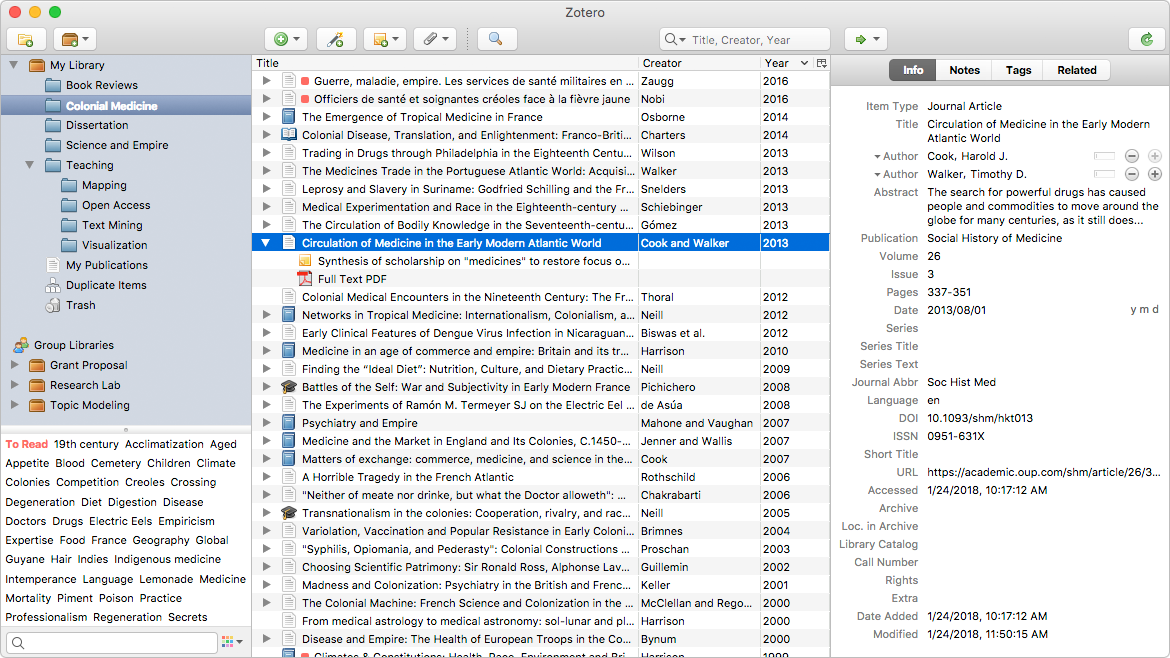
\includegraphics[width=0.8\textwidth]{pictures/zotero.png}
\caption{Zotero基本界面}
\label{fig566}
\end{figure}




\paragraph{(1)常用的功能}
如图(\ref{fig566})所示,Zotero基本分成三栏,左边是分类区,中间是文献区,右边是文献详细信息区。
分类区又分为上下两区,上面称为 Collection,下面则是每篇文献的标签汇总称为Tag。
\begin{itemize}
\item 前往官网下载安装相应版本和插件,并注册帐号。
\item 在 Library 创建 Collection。
\item 选中 Collection 就可以在程序中间文献区导入文献,这样 Zotero 就自动获取文献名、作者、年份等信息。导入文献有两种方式:
\begin{itemize}
\item Link to File: 这种是建立与本地文献链接,不上传到云盘模式。
\item Store Copy of File: 这种是复制到Zotero存贮区上传到云盘模式。请参考多平台、多设备同步。
\end{itemize}
\item 选择一篇文献,在右侧Tags处写上标签,一般多个,如:特别关注的作者、文献中的方法和研究对象。
\item 所有标签就会出现在 第一栏下面区域。首先在 Collection 区域选择 Library,中栏就能呈现所有文献,再在 Tag 区域选中任意标签,就会在中栏筛选出相应的标签。选中多个标签,则是取文献的交集。
\item 通过标签解决了一篇文献多个分类的问题。
\item Collection 中的文献复制有两种方式:
\begin{itemize}
\item 选中 + 拖放:在多个Colletion中复制并保留文献条目; 
\item 选中 + shift + 拖放:从不同Colletion中移动条目。
\end{itemize}
\end{itemize}



\paragraph{(2)文献快速下载与导入}
通过相关的浏览器插件,可以一步实现文献下载和Zotero的导入。但是前提的有,1)Zotero是打开着的;2)自己有文献下载的权限,能把文献下载下来,如果不能,则只会保存一个文献信息,需要后期关联。



\paragraph{(3)多平台、多设备同步}
这是一个非常实用的功能。

\emph{以我为例,主要工作系统是 Ubuntu 系统。但为了实现无纸化办公,我喜欢用微软的 Surface 来阅读文献。而且用 Surface 的笔可以直接在pdf文献上标注,标注也可以同步到主要工作电脑上,非常方便。}

Zotero 自己是有空间同步本地文献的,但是价格太贵。主要可以采用两种方式:1)Zotero +同步盘(任意云盘,软链接);2)Zotero +坚果云WebDAV。推荐后者,详情请参考青柠学术微信公众号专辑,Zotero|打造最佳文献生态。

\paragraph{(4)文献全文检索并自动更新}
还是参考青柠学术Zotero专辑。在“My library”右键有“New Saved Search”。这个可以对文献库中文献进行特定检索,并随着加入的文献自动更新。



\subsection{文献下载}
\begin{itemize}
\item \url{https://bookos-z1.org/}:英文专业书籍下载网站
\item \url{https://iseex.github.io/ScholarNavi}:文献下载网站
\item Zotero + Zotero Connector + Zotero-shortdoi + SCi-Hub: 文献下载标签一条龙,几乎能完成99\%文献下载,参考青柠学术的Zotero专题。
\end{itemize}

\begin{itemize}
\item \url{https://mp.weixin.qq.com/s/q7fZJVZbFaL_xwtRxivD2w}
\item \url{https://iseex.github.io/2020-03/zotero-shortdoi/}
\end{itemize}


\subsection{文献检索与跟踪——Google学术}
参考:\url{https://scholar.google.com/intl/en/scholar/help.html#overview}

\url{https://iseex.github.io/2020-04/zotero-rss-papers-subscription}



\subsection{Pdf批量全文搜索工具——Recoll}
\begin{itemize}
\item Recoll 网址:\url{https://www.lesbonscomptes.com/recoll/}

\item 参考网址:\url{http://www.linuxdown.net/install/faq/20160318_how_linux_5065.html}
\end{itemize}


\subsection{文献阅读}
文献阅读有两种状态:浏览(泛读)和精读。

\paragraph{文献浏览}旨在了解最新发展动态,激发科研想法。应该保持每天一定时间不限量的浏览。






\section{科研资源}
\subsection{光学相关}
 \begin{itemize}
\item \url{http://toolbox.lightcon.com/}
\end{itemize}


\section{自然科学论文写作}
\subsection{摘要(Abstract)}
摘要一般5到6句话。
\begin{itemize}
\item 第一句:大背景;
\item 第二句:领域中有什么问题、我想做什么、有什么是未知的、有什么需要做的;
\item 有些文章不写第一句、第二句
\item 第三句:我用什么方法研究了什么东西;
\item 第四、五句:有什么结果。或加一句分析一下;
\item 最后一句:意义(重要性)。
\end{itemize}


\subsection{引言(Introduction)}
引言的写作直接影响到读者对文章进一步了解的兴趣, 建议包括以下内容\footnote{参考自物理学报的投稿模板}:
\begin{enumerate}
\item 本研究领域背景的综述;
\item 其他学者已有研究成果的详细描述;
\item 陈述为什么需要进行更多的或进一步的研究;
\item 阐述作者本项研究的目的和创新性;
\item 简述本文开展的研究工作;
\item 本项研究结果的意义(可选项)。
\item 特别指出的是, 希望在引言部分介绍和引用国内外期刊中本研究领域的最新研究成果, 以帮助读者清楚了解该领域的最新进展及本文的创新点。
\end{enumerate}



\section{演示文稿制作}
图和列表(关键词)



\section{墙报制作}








\chapter{国家自然科学基金申请书的写作}
参考资料:一些讲座、同事老师经验和自己的体会。【不注明出处】
\section{思想层面}
\subsection{基本认识——“向国家要钱”}
\begin{itemize}
\item 基础科研可以说是没有直接经济产出的。未来也是可能有也可能没有,而且时间也是长短不一,一般很长。所以基础科研不挣钱的。
\item 但是科研又是需要钱的。所以需要去“要”钱。向“谁”要?
\item 向“别人”要钱,所以要按人家要求来,要说服“别人”。
%很难自己对什么感兴趣,就研究什么。
\end{itemize}


\subsection{国家和自己的定位}
\paragraph{国家基金的定位}
\begin{itemize}
\item 基础研究(不是工程问题)。
\item 基金不是产品开发,基金是解决局部问题,局部的基础科学问题研究。
\end{itemize}

\paragraph{自己的定位}
\begin{itemize}
\item 国家需求的一小点
\item 交叉学部(注意交叉融合)
\end{itemize}


\subsection{指导思想}
\begin{itemize}
\item 如何写好一个本子?解决一个问题,讲好一个故事。

\item 基金如战事,“谋”则胜:认真谋划,积极请教,提前布局,方得始终。

\item 不可打酱油心态,要不断打磨本子。

\item 广结善缘:评阅人先看论文,再看人。文章->团队出身->内容。注意选口。
\end{itemize}


\subsection{基本认识}
\begin{itemize}
\item 千万不要有标点符号等错误。
\item 专家在挑刺,10分钟看本本。
\item 让大同行看懂,让小同行似懂非懂。
\item 系统送审,大同行评审(小学校、年青老师)。
\item 关键词要选好,评阅人通过关键词分配。
\end{itemize}


\subsection{整体思路}
\begin{itemize}
\item 立项依据非常重要。
\item 借文献说出不足之处。
\item 千万不要太细。
\item 可行性分析起打补丁的作用。
\item 修补性创新(改进型)。
\item 研究基础与工作条件(注意合作单位;人不够,合作很关键;个人基础薄弱,团队很重要。)
\item 图文并茂,图就在图注中解释,不用在正文中解释。
\item 小四号,1.5倍行距,楷体。
\end{itemize}


\paragraph{三要素}
\begin{enumerate}
\item 研究对象
\begin{itemize}
\item 研究主体是什么?
\item 应用的领域是否重要?
\item 存在的问题是否为痛点问题?
\end{itemize}

\item 需要解决的问题

\item 解决问题的方法:科学方法
\end{enumerate}


\paragraph{说清楚三个问题}
\begin{enumerate}
\item 项目研究的内容值得做;
\item 项目研究的内容能够做好; 
\item 项目研究的内容我能做的更好。
\end{enumerate}

\paragraph{如何做到?}
选题极为关键,申请书撰写规范极为重要,创新性和科学性决定成败。


\section{参考资源}
\begin{itemize}
\item 国家自然科学基金网站
\item 国家服务平台(大数据平台)
\item 科学网基金板块
\end{itemize}


\section{时间点与安排}
\begin{itemize}
\item 选题是基金成败关键,提前半年,初申请者最好提前一年进行选题调研,要有一定的预研
\item 充分构思,快速初稿,细致修改,每天揣摩
\item 9月底有草稿,10月有初稿
\item 5天内完成初稿
\item 1月解读指南
\end{itemize}



\section{具体写作层面}
\subsection{选题}
\begin{itemize}
\item 选题应以问题为导向,不要以方法为导向。拿着所谓的“新方法”去找应用场景,由于对研究主体说不清道不明,往往被从根上被判为是“伪命题”。

\item 科学问题不要包罗万象,解决系统的所有问题。要“小题深做”,往下挖掘,不是面面俱到。

\item 尚未解决或新生的科学问题(聚焦到一个点或两个点,注意交叉创新)

\item 挑选有“吸引眼球”的应用领域非常重要。
	\begin{itemize}
	\item 同样的科学问题可以应用到不同领域
	\item 应用领域要拔高
	\end{itemize}
\item 方法源于问题。
\end{itemize}



\subsection{标题}
\begin{itemize}
\item {\color{red} 从题目中要能看出本本的轮廓。}

\item 理清楚了基金的三个基本要素,取名字时要集中体现三个基本要素。要求:名字中要明确研究对象、明确要解决的问题、明确采用的方法(或者突出特殊条件),比如:基于XX方法的XX对象XXX问题研究;或者:某种特点条件下某研究对象的什么问题研究。

\item 忌讳名字大而空,忌讳:某某关键技术的研究、某某重大技术的研究、某某系统的研究等;基金是基础研究,不是技术研究,也不是应用研究,名字中尽量不要突出技术或应用。

\item 好标题:具体、新意、务实

\item 研究对象是个名词,对象要具体。面上、青年研究某个关键问题。

\item 题目由:对象、问题、方法构成,惟一可缺的是方法。
\end{itemize}




\subsection{摘要}
\begin{itemize}
\item {\color{red}从摘要能看出申请书的骨骼构架,它包含:背景及问题、目标、内容、意义。}
\item 摘要要吸引人,眼前一亮,新的东西
\end{itemize}

写一个精炼的摘要,做到多一字则多,少一字则没表达清楚。要求:
\begin{itemize}
\item 第一句话:研究对象的背景及存在的问题;(领域背景问题)
\item 第二句话:本项目拟采用什么方法解决哪些问题;(研究目标)
\item 第三句话:解决问题的具体内容;(研究内容)
\item 最后一句话:问题解决对所在领域的理论和现实意义。(研究意义)
\end{itemize}

摘要的书写规范概况起来:
\begin{itemize}
\item 本项目研究的东西在某个领域里至关重要,但是它存在某些问题需要解决。
\item 本项目拟采用某某方法来解决这个问题。
\item 具体的内容如下:
	\begin{itemize}
	\item[1)] 先做什么;
	\item[2)] 再做什么;
	\item[3)] 最后怎么样验证的,得到啥结论。
	\end{itemize}
\item 某某问题的解决对某某领域的某项技术的发展提供理论支持。
\end{itemize}



\subsection{项目的立项依据}
(研究意义、国内外研究现状及发展动态分析,需结合科学研究发展趋势来论述科学意义;或结合国民经济和社会发展中迫切需要解决的关键科技问题来论述其应用前景。附主要参考文献目录);

\paragraph{指导思想}
\begin{enumerate}
\item 国内外研究现状及分析要准确,中庸,绝不能偏激。
\item 不谈历史,不谈产品,不谈某某公司做了什么事,只谈近3-5年研究对象及其存在的问题,并且是科学问题,不是简单的技术革新。
\item 让专家阅读欣赏你的申请书,不要让专家琢磨研究你的申请书。
\item 写基金申请书和建筑设计院设计大楼是一样的,设计院要把大楼的各个细节完全设计好了,甲方才会投钱施工。同样,基金的各个环节也必须落地,完全规划好,不能空洞。基金的整个过程就是编故事,要能够自圆其说,落脚踏实。
\item 任何重要的论点都要有文献标注,有文献就等于没有疑问。参考文献要新,最好是当年的。而且一定要引上本学科主流杂志的近期文献,增加自己理论依据的权威性。国内小同行里的知名学者的成果要适当引用,但不能批驳,要婉转的表达你是在他的基础上走一步,而不能否定他的成果。
\end{enumerate}


\subsubsection{项目的研究意义(剥洋葱写法)}
\begin{itemize}
\item 第一段:研究对象在其所在领域有重要的理论或应用价值,研究对象“因具有哪些优点而被关注或应用,但因存在哪些问题而需要进一步研究”,突出三个东西:领域重要、对象是关键部件、痛点问题迫切需要解决。(300字以内)

\item 第二段:痛点问题产生的原因是什么?挖掘出问题的根源,找出解决问题的难点,从众多难点中,理清难点间的逻辑关系,突出最核心的问题。(200字左右)

\item 第三段:核心问题的解决方法当前有哪些,各有何优缺点,当前核心问题的解决方法存在什么科学问题。(200字左右)

\item 第四段:本项目解决该问题需要研究的一至两个核心科学问题(非技术问题)。(200字)

\item 第五段:鉴于上述分析,本项目以解决研究对象的什么问题为目的,通过什么方法实现该科学问题的解决,在某领域具有重要的理论意义和实践价值。(150字)

\item 总篇幅:正文第一页到第二页前10行。

\item {\color{red} 这部分写好了,能看出申请书的经络关系。}
\end{itemize}


\subsubsection{国内外研究现状及分析}
这个部分要分析三个层面的现状:
\begin{itemize}
\item 1.2.1、研究对象的现状;
\item 1.2.2、该对象存在的问题的现状;
\item 1.2.3、解决问题的方法的现状;
\item 1.2.4、本项目解决问题的思路和亮点。
\item 注意小标题的应用,小段落、一段一事、每段不超过8行。
\item 以分析为框架,以文献做佐证,抽调文献,分析还自成体系。
\end{itemize}


\subsubsection{主要参考文献}
\begin{itemize}
\item 数量:30左右;
\item 时间:3年之内,务必要有当年的;
\item 来源:国内外有重要影响的期刊;
\item 语种:英文居多;
\item 作者:本学科知名小同行的文章;
\item 格式:格式完全统一,不要简单复制堆砌。
\end{itemize}



\subsection{项目的研究内容、研究目标,以及拟解决的关键科学问题【研究方案的撰写】}
(此部分为重点阐述内容);
\subsubsection{研究目标}
总体目标:本项目针对研究对象存在的什么问题,拟采用什么方法,通过哪几个方面的研究,实现问题的解决,关键点的阶段性目标如下:
\begin{itemize}
\item[1)] 目标1:采用什么方法,解决什么问题,达到什么效果;
\item[2)] 目标2:采用什么方法,解决什么问题,达到什么效果;
\item[n)] 目标3:采用什么方法,解决什么问题,达到什么效果;
\end{itemize}


\subsubsection{研究内容}
\begin{itemize}
\item[1)] 研究内容要集中,与研究目标紧密一致,说的是众难点问题解决要做什么事,一条研究内容,解决一个难点;

\item[2)] 研究内容4条左右即可,每条论述150-200字为宜,且对各点的内容不要展开论述,主说针对什么子问题,拟采用什么方法做什么事,怎么做的,不说。

\item[3)] 各研究内容的逻辑关系是递进的,不能是平行的。

\item 格式:一个醒目的完整的小标题,加粗加黑,5-8行字的内容。主要写针对什么目标,拟采用什么方法解决该问题。

\item {\color{red} 这部分写好了,就能开出申请书的肌肉了。}
\end{itemize}


\subsubsection{拟解决的关键科学问题(非常重要)}
\begin{itemize}
\item[1)]  关键科学问题不是研究内容的简单重复,是项目一开始就凝练出的核心科学问题;(研究意义的第四段)

\item[2)] 如果说研究内容是说采用某方法解决某难点问题,拟解决的关键科学问题就是对采用的方法如何进行科学性创新,才能使难点问题得到科学的解决。

\item 关键科学问题要落地,要说得清道得明,不是简单的画大饼,不是笼统的说要研究什么机理,什么规律。
\end{itemize}





\subsection{拟采取的研究方案及可行性分析}
(包括研究方法、技术路线、实验手段、关键技术等说明);
\subsubsection{研究方法}
本项目针对什么问题,从系统分析、理论分析、仿真验证和实验验证等方面开展什么研究对象的什么关键问题的研究。
\begin{itemize}
\item 系统分析方面:每一点写3行以内
\item 理论研究方面:
\item 仿真验证方面:
\item 实验研究方面:
\end{itemize}
每一点写3行以内,不展开,突出统筹逻辑和方法的新。


\subsubsection{项目的技术路线}
\begin{itemize}
\item[1)] 研究意义是说为什么做,研究内容是说做什么,而技术路线就是要说怎么做了。

\item[2)] 研究意义、研究内容、拟解决的科学问题都是要求大家言简意赅,不要展开,那到了技术路线部分,就要完全展开了。

\item[3)] 技术路线的格式:
\begin{itemize}
\item 先写一个总体的路线概括,约200字(约5行),主要介绍项目采用什么方法,分别要解决那几个主要内容,类似于立项依据的总结部分,但是表述方式有所不同。

\item 再画一个技术路线的总体框图,集中体现了研究内容的各个模块,每个模块中要有解决问题的方法要点。

\item 各模块之间最好是顺序流程,一目了然,切忌模块之间穿插太多。主线部分顺序明确,自上而下,理论分析辅助部分和实验验证部分分列两侧。

\item 展开论述各环节实施方案,有分析、有理论指导,有图,充分展示。

\item 小标题呼应研究内容“XXXX的实施路线”,每个小标题展开一个以内。例如
	\begin{itemize}
	\item 3.2.1 研究内容一(用具体内容)的实施路线
	\item 3.2.2 研究内容一(用具体内容)的实施路线
	\item 3.2.3 研究内容一(用具体内容)的实施路线
	\item 3.2.5 搭建什么样的实验平台,开展什么样的实验研究。
\end{itemize}
\end{itemize}
\item 这部分写好了,就能看出申请书“皮肤包裹之下的驱壳和灵魂了”。
\end{itemize}


\subsubsection{实验手段}
本项目结合XXXX的需求,搭建了什么样的实验平台,开展如下实验研究:
\begin{itemize}
\item 仿真实验
\item 半实物仿真实验研究
\item 样机实验研究
\end{itemize}


\subsubsection{关键技术}
关键技术不是关键科学问题,是为了实现研究内容,在技术方案实施中,支持方案完成的核心技术问题。


\subsubsection{可行性分析}
可行性分析分三个层面来写:
\begin{itemize}
\item[一、]理论与技术上可行,介绍项目所用理论在相同或相近问题上解决的先例;
\item[二、]实验条件可行,本单位现有技术设备实验材料的完备,能够满足实验要求;
\item[三、]知识技能上可行,课题组人员结构,知识储备等具备完成课题的能力。
\end{itemize}


\subsection{本项目的特色与创新之处;}
\begin{itemize}
\item[1)] 原理性创新;
\item[2)] 引入型创新:马克思主义引入中国,和不同时期的中国具体国情相结合,分别产生了毛泽东思想、邓小平理论及习近平新时期思想。
\item 这部分写好了,类似于能看清楚一个人的品德优点了。
\end{itemize}



\subsection{年度研究计划及预期研究结果}
(包括拟组织的重要学术交流活动、国际合作与交流计划等)。
\begin{itemize}
\item 2022年1月-2022年12月;
\item 2023年1月-20023年12月
\item ....
\item 日期和前面起始日期完全对应,不能错一天,否则初筛就出局了。
\end{itemize}

预期研究结果

一个模式作参考:
\begin{itemize}
\item[1)] 呼应研究内容:探索一种XXXX方法,研究XXXX算法,形成XXXX的理论方法和实现手段。

\item[2)] 在国内外权威期刊上发表论文3-5篇,并被SCI或EI收录3-5篇。

\item[3)] 培养博士生1-2名,培养硕士生3-5名。
\end{itemize}



\subsection{研究基础与工作条件}
\subsubsection{工作基础}
(与本项目相关的研究工作积累和已取得的研究工作成绩);
\paragraph{1.1 申请团队的研究背景}
一句话介绍课题组依托的实验室(有影响力的,没影响力的就不要写了),申请人或课题组近年来研究方向,取得的阶段性成果,简单介绍一下,课题组人员的搭配等。重点是下一个环节。

\paragraph{1.2 在本项目研究工作积累和已取得的研究工作成绩}
\begin{itemize}
\item[1.2.1] 研究内容1方面的工作积累
	\begin{itemize}
	\item 3-5行概况该方面的工作
	\item 三张图(样机、分析过程图、实验图等)
	\item 论文专利
	\end{itemize}
	
\item[1.2.2] 研究内容2方面的工作积累
	\begin{itemize}
	\item 3-5行概况该方面的工作
	\item 三张图(样机、分析过程图、实验图等)
	\item 论文专利
	\end{itemize}
	
\item ...
\end{itemize}
申请人或课题组近5年来做了哪些和本项目研究对象直接或间接相关的事情,逐个介绍,并配一些有标注的图。


\paragraph{1.3 与本项目直接相关的代表性学术论文}
列举近5年来课题组发表的和本项目直接相关的论文,关联度最近的写在前面,质量最高的写在前面。太差的期刊就不要写了,选择有代表性的。

这部分写好了,就能够看出这个人的血统和出身了。


\subsubsection{工作条件}
(包括已具备的实验条件,尚缺少的实验条件和拟解决的途径,包括利用国家实验室、国家重点实验室和部分重点实验室等研究基地的计划与落实情况);

申请人在本项目方向上的研究依托哪些有影响的实验室,该实验室具备哪些软硬件条件能够支撑本项目的开展。然后分开写:
\begin{itemize}
\item 硬件方面:
\item 软件方面:
\end{itemize}



\subsubsection{正在承担的与本项目相关的科研项目情况}
(申请人和项目组主要参与者正在承担的科研项目情况,包括国家自然科学基金的项目,要注明项目的名称和编号、经费来源、起止年月、与本项目的关系及负责的内容等);

注意:主要指基金项目



\subsubsection{完成国家自然科学基金项目情况}
(对申请人负责的前一个已结题科学基金项目(项目名称及批准号)完成情况、后续研究进展及与本申请项目的关系加以详细说明。另附该已结题项目研究工作总结摘要(限500字)和相关成果的详细目录)。

有就写,没有就写无。



\subsection{申请人和项目组主要参与者简介(在读研究生除外)。}
说明:在职教师的硕士博士博士后导师必须写,不写直接出局



\subsection{经费申请说明}
购置单项经费5万元以上固定资产及设备等,须逐项说明与项目研究的直接相关性及必要性。

最好不要买5万元以上的设备,写了说明你的实验室条件不具备。



\section{落选的原因}
\begin{enumerate}
\item 没理清楚三要素;
\item 写的东西让人看着累,不想看了;
\item 创新性工作不突出、研究重点不突出;
\item 关键科学问题没挖掘到位;
\item 技术路线没展开,没有解决问题的方法和措施;
\item 研究基础显得不扎实。
\end{enumerate}










